\documentclass[12pt, a4paper]{article}
\usepackage[czech]{babel}

\usepackage{graphicx}
\usepackage{parskip}
\usepackage{longtable}
\usepackage{amsmath}
\usepackage{float}
\usepackage{url}
\usepackage{microtype}
\usepackage{multirow}
\usepackage{tabularx}
\usepackage[margin=2cm]{geometry}

\usepackage[backend=biber,style=authoryear]{biblatex}
\addbibresource{zdroje.bib}

\begin{document}

\begin{titlepage}
    \centering
    {\large UNIVERZITA KARLOVA\par}
    \vspace{0.2cm}
    {\large {Přírodovědecká fakulta}\par}
    \vspace{0.2cm}
    {\large Katedra aplikované geoinformatiky a kartografie\par}

    \vspace{2cm}

    {\large Studijní program:\par}
    \vspace{0.2cm}
    {\large Geoinformatika, kartografie a dálkový průzkum Země\par}

    \vspace{2cm}

    
\includegraphics[width=5cm]{logo.png}\par

    \vspace{1cm}

    {\large \textbf{Jakub Fuchsig, Šimon Kohout}\par}
    \vspace{1cm}
    {\Large \textbf{Úloha 1: Výpočet souřadnic bodů v rovině Křovákova zobrazení}\par}
    \vspace{2cm}  
    {\large Ústí nad Labem, Zákupy\par} 
\end{titlepage}
\clearpage
\newpage

\section*{Zadání}

GPS aparaturou změřte zeměpisné souřadnice bodu, A bodů $P_{1}$ $P_{2}$ vztažené k elipsoidu WGS-84 a vypočtěte $\varphi$ jejich obraz v rovině Křovákova zobrazení.

Měření proveďte na bodech o známých souřadnicích (trigonometrický bod), a to opakovaně.

Pro transformaci mezi elipsoidy použijte sedmiprvkovou Helmertovou prostorovou podobnostní transformaci danou vztahem
\begin{equation*}
\begin{pmatrix} X \\ Y \\ Z \end{pmatrix} = m \begin{pmatrix} 1 & \omega_{z} & -\omega_{y} \\ -\omega_{z} & 1 & \omega_{x} \\ \omega_{y} & -\omega_{x} & 1 \end{pmatrix} \begin{pmatrix} X^{\prime} \\ Y^{\prime} \\ Z^{\prime} \end{pmatrix} + \begin{pmatrix} \Delta X \\ \Delta Y \\ \Delta Z \end{pmatrix}.
\end{equation*}

Parametry prostorové transformace:

\vspace{1em}
\begin{center}
\begin{tabular}{|l|l|}
\hline
$\omega_{x}$ & $4.9984^{\prime\prime}$ \\ \hline
$\omega_{y}$ & $1.5867^{\prime\prime}$ \\ \hline
$\omega_{z}$ & $5.2611^{\prime\prime}$ \\ \hline
$m-1$ & $-3.5623e^{-6}$ \\ \hline
$\Delta X$ & $-570.8285$ m \\ \hline
$\Delta Y$ & $-85.6769$ m \\ \hline
$\Delta Z$ & $-462.8420$ m \\ \hline
\end{tabular}
\end{center}
\vspace{1em}

Určení zeměpisné šířky obrazu bodu P na Besselově elipsoidu proveďte s přesností 0.001". Souřadnice obrazu bodu P v rovině Křovákova zobrazení určete s přesností na cm. V bodech $P_{1}$ $P_{2}$ dále vypočtěte:

\begin{itemize}
    \item hodnoty délkového zkreslení $m-1$,
    \item hodnoty meridiánové konvergence c.
\end{itemize}

Volitelně porovnejte účinek zanedbání změny/vlivu elipsoidu na souřadnice bodů $P_{1}$, $P_{2}$ a na vzdálenosti $||P_{1}-P_{2}||$.

Jak se budou lišit takto určené souřadnice a vzdálenosti od hodnot vztažených k elipsoidu WGS-84?

Obrazy bodů $P_{1}$, $P_{2}$ a jejich blízkého okolí vizualizujte s použitím vhodných podkladových geografických dat (např. WMS).

Výpočty realizujte v SW Matlab.

\vspace{1.5em}
\noindent\textbf{Hodnocení:}
\vspace{1em}

\begin{center}
\begin{tabular}{|p{12.5cm}|c|}
\hline
\textbf{Krok} & \textbf{Hodnocení} \\ \hline\hline
Výpočet souřadnic bodu v rovině Křovákova zobrazení + zkreslení. & 20b \\ \hline
Výpočet meridiánové konvergence & +5b \\ \hline
\textbf{Max celkem:} & \textbf{25b} \\ \hline
\end{tabular}
\end{center}

\clearpage
\newpage

\section{Úvod}
Tato práce se zabývá problematikou exaktního převodu geodetických dat mezi globálním referenčním systémem a národním souřadnicovým systémem. Konkrétním úkolem je transformace zeměpisných souřadnic bodů $P_1$ a $P_2$, získaných pomocí technologie GNSS (Global Navigation Satellite Systems) v systému WGS-84, do roviny Křovákova zobrazení, které definuje souřadnicový systém Jednotné trigonometrické sítě katastrální (S-JTSK).

Tento proces není pouhou lineární transformací, ale představuje komplexní řetězec matematických operací, které musí zohlednit odlišné parametry referenčních elipsoidů (WGS-84 a Besselův elipsoid 1841) i geometrické vlastnosti následných kartografických zobrazení. Klíčovým prvkem je zde sedmiprvková Helmertova prostorová transformace, která řeší nesouosost a odlišné měřítko obou geocentrických systémů.

Vlastní kartografická část úlohy pak spočívá v realizaci dvojitého konformního zobrazení. Prvním krokem je Gaussovo zobrazení Besselova elipsoidu na referenční kouli (tzv. Gaussovu kouli). Následně je využito Lambertovo konformní kuželové zobrazení v obecné poloze, které převádí body z koule do roviny. Specifikem Křovákova zobrazení je volba kartografického pólu a orientace souřadnicových os, což zajišťuje minimální zkreslení pro území bývalého Československa.

Kromě samotného výpočtu souřadnic $[Y, X]$ je cílem práce také analytické vyhodnocení kvality zobrazení v daných lokalitách, konkrétně výpočet lokálního délkového zkreslení a meridiánové konvergence. V neposlední řadě se práce zaměřuje na analytické porovnání přesného výpočetního postupu s jeho zjednodušenými variantami. Cílem této části je kvantifikovat odchylky v souřadnicích a prostorových vzdálenostech, které vznikají při záměrném zanedbání změny referenčního elipsoidu (přímé použití souřadnic WGS-84 na tělese Besselova elipsoidu). Tento rozbor je klíčový pro stanovení mezí přesnosti a určení měřítek mapové dokumentace, u nichž jsou taková matematická zjednodušení v inženýrské praxi ještě přípustná.

\section{Vstupní data a jejich zpracování}

V souladu se zadáním úlohy č. 1 byla měření zeměpisných souřadnic provedena pomocí GPS aparatury (technologie GNSS). Aby bylo možné v závěru práce provést korektní analýzu přesnosti transformace, byla měření vztažena k existujícím bodům podrobného polohového bodového pole (PPBP) o známých souřadnicích.

Pro účely této práce byly vybrány dvě lokality na území hlavního města Prahy:
\begin{itemize}
    \item \textbf{Bod $P_1$ (Albertov):} Vztažen k geodetickému bodu č. 569 (k. ú. Nové Město). Bod je definován jako jihovýchodní roh domu č. p. 2049.
    \item \textbf{Bod $P_2$ (Střížkov):} Vztažen k geodetickému bodu č. 568 (k. ú. Střížkov). Bod se nachází u regulační stanice plynu v ulici Lovosická.
\end{itemize}

Níže jsou zobrazeny širší lokalizace obou bodů v mapovém podkladu (obr. \ref{fig:lokalizace1} a \ref{fig:lokalizace2}).

\begin{figure}[h!]
    \centering
    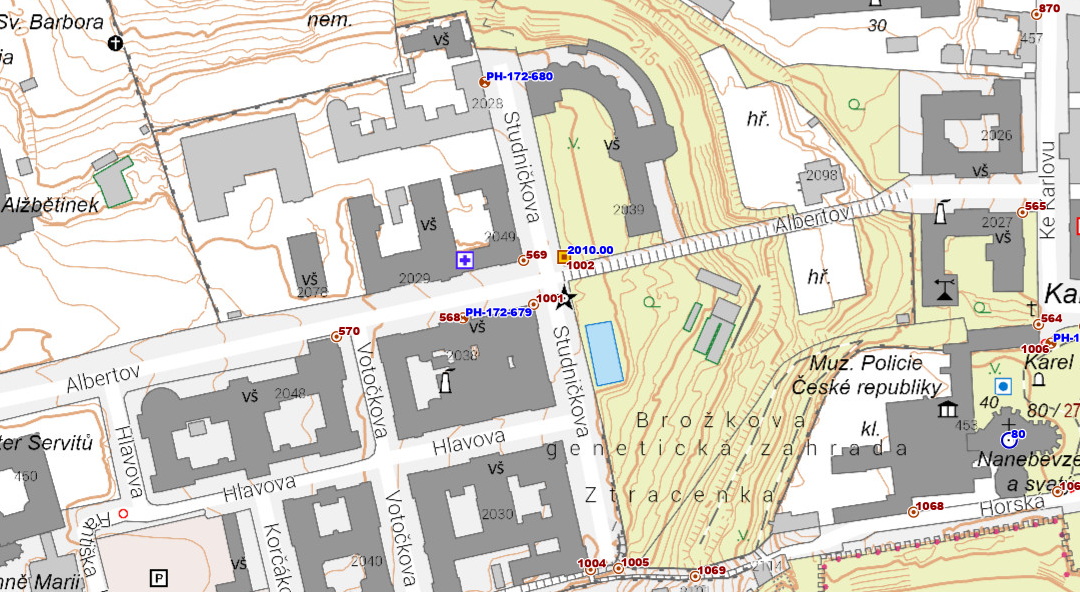
\includegraphics[width=1\textwidth]{569.png}
    \caption{Poloha bodu č. 569 na Albertově.}
    \label{fig:lokalizace1}
\end{figure}

\begin{figure}[h!]
    \centering
    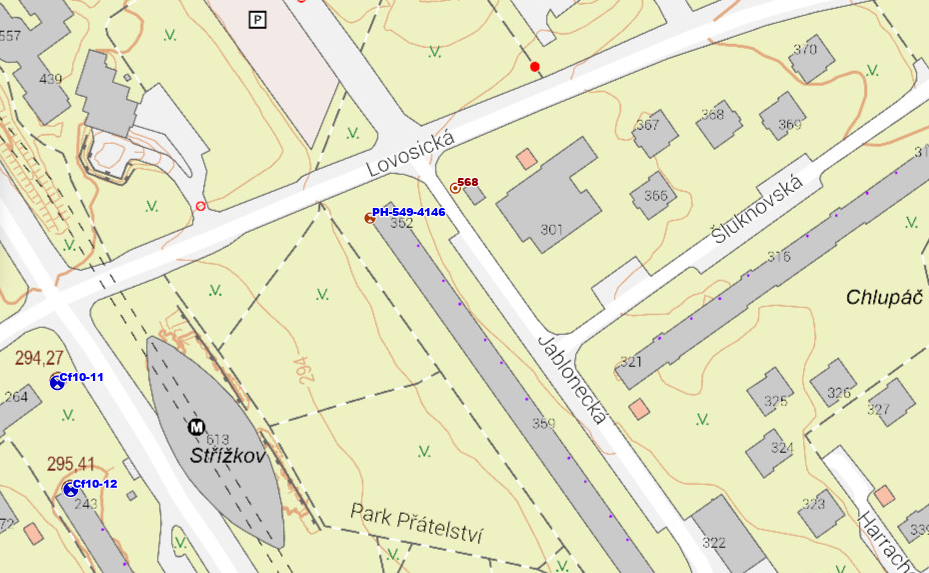
\includegraphics[width=1\textwidth]{568.png}
    \caption{Poloha bodu č. 568 na Střížkově.}
    \label{fig:lokalizace2}
\end{figure}

\subsection{Místopisné náčrtky bodů PPBP}
Pro jednoznačnou identifikaci v terénu byly využity oficiální geodetické údaje. Místopisné náčrtky (obr. \ref{fig:nacrt569} a \ref{fig:nacrt568}) znázorňují přesnou stabilizaci bodů a jejich vazbu na okolní objekty pomocí oměrných měr.

\begin{figure}[h!]
    \centering
    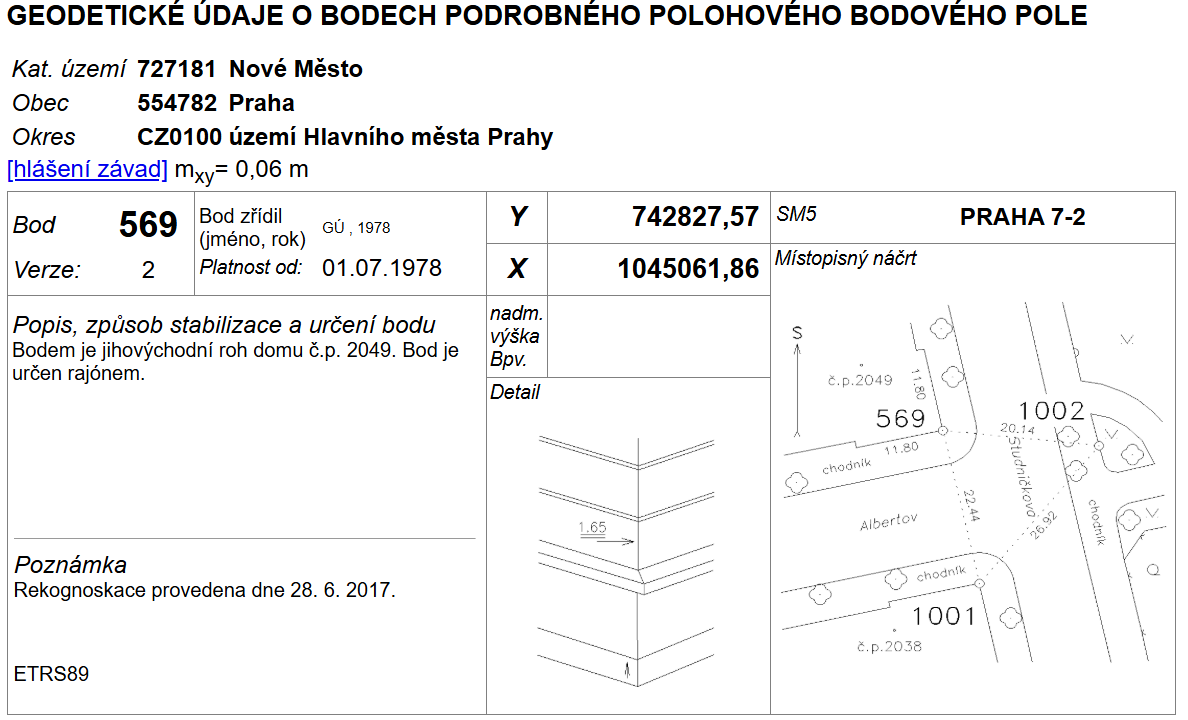
\includegraphics[width=1\textwidth]{Albertov.png}
    \caption{Místopisný náčrt bodu č. 569 (Albertov).}
    \label{fig:nacrt569}
\end{figure}

\begin{figure}[h!]
    \centering
    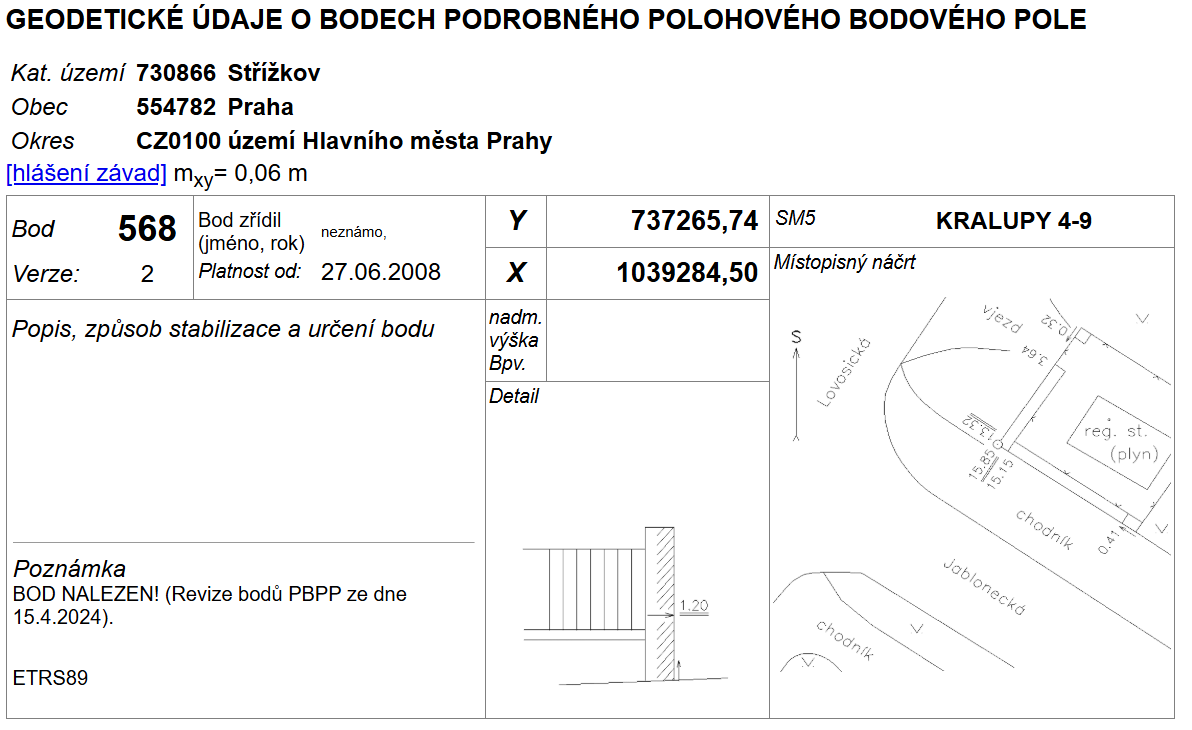
\includegraphics[width=1\textwidth]{Strizkov.png}
    \caption{Místopisný náčrt bodu č. 568 (Střížkov).}
    \label{fig:nacrt568}
\end{figure}

\clearpage
\newpage


\subsection{Statistické zpracování měření}
Aby se minimalizoval vliv náhodných chyb GPS měření, bylo na každém stanovišti provedeno měření opakovaně ve třech sadách. Pro další výpočty byl z těchto hodnot stanoven aritmetický průměr. Naměřené souřadnice vztažené k elipsoidu WGS-84 jsou uvedeny v tabulkách \ref{tab:P1} a \ref{tab:P2}.

\begin{table}[h!]
\centering
\begin{tabular}{|c|c|c|}
\hline
\textbf{Sada měření} & \textbf{Zeměpisná šířka $\varphi^\circ$} & \textbf{Zeměpisná délka $\lambda^\circ$} \\ \hline
1 & 50.0691914 & 14.4249158 \\ \hline
2 & 50.0691890 & 14.4249145 \\ \hline
3 & 50.0691931 & 14.4249169 \\ \hline\hline
\textbf{Průměr ($P_1$)} & \textbf{50.06919117} & \textbf{14.42491573} \\ \hline
\end{tabular}
\caption{Měření na Albertově ($P_1$).}
\label{tab:P1}
\end{table}

\begin{table}[h!]
\centering
\begin{tabular}{|c|c|c|}
\hline
\textbf{Sada měření} & \textbf{Zeměpisná šířka $\varphi^\circ$} & \textbf{Zeměpisná délka $\lambda^\circ$} \\ \hline
1 & 50.1274507 & 14.4909381 \\ \hline
2 & 50.1274351 & 14.4909124 \\ \hline
3 & 50.1274426 & 14.4909504 \\ \hline\hline
\textbf{Průměr ($P_2$)} & \textbf{50.12744280} & \textbf{14.49093363} \\ \hline
\end{tabular}
\caption{Měření na Střížkově ($P_2$).}
\label{tab:P2}
\end{table}

Zpracování dat probíhalo v jazyce Python. Následující úryvek kódu ukazuje metodu průměrování a převod na radiány, přičemž blok je v reportu vycentrován pro lepší přehlednost:

\vspace{0.5cm}
\begin{center}
\begin{minipage}{0.7\textwidth}
\begin{verbatim}
# Average of measurements
phi_WGS = (u11 + u12 + u13) / 3 * pi/180
la_WGS = (v11 + v12 + v13) / 3 * pi/180

phi_WGS2 = (u21 + u22 + u23) / 3 * pi/180
la_WGS2 = (v21 + v22 + v23) / 3 * pi/180
\end{verbatim}
\end{minipage}
\end{center}


\section{Matematický model Křovákova zobrazení a transformace souřadnic}
Převod měřených souřadnic z referenčního elipsoidu WGS-84 do roviny Křovákova zobrazení (S-JTSK) sestává z několika na sebe navazujících kroků, které zahrnují změnu referenčního tělesa i následné dvojité konformní zobrazení. 

\subsection{Vztah zeměpisných a geocentrických souřadnic}
Prvním krokem je převod zeměpisných souřadnic $[\varphi', \lambda']$, vztažených k elipsoidu WGS-84, na prostorové geocentrické souřadnice $[X', Y', Z']$ vztažené k témuž elipsoidu. Bod $P'$, u kterého předpokládáme nulovou elipsoidickou výšku, je v 3D prostoru definován vztahem:

$$P' = \begin{pmatrix} X' \\ Y' \\ Z' \end{pmatrix} = N \begin{pmatrix} \cos \varphi' \cos \lambda' \\ \cos \varphi' \sin \lambda' \\ (1 - e^2) \sin \varphi' \end{pmatrix}$$

kde $N$ představuje příčný poloměr křivosti:
$$N = \frac{a}{W}$$

Hodnota $W$ reprezentuje první geodetickou funkci:
$$W = \sqrt{1 - e^2 \sin^2 \varphi'}$$

Parametr $e^2$ je první excentricita elipsoidu, která se vypočte z hlavní poloosy $a$ a vedlejší poloosy $b$:
$$e^2 = \frac{a^2 - b^2}{a^2}$$

\subsection{Prostorová podobnostní transformace (Helmertova)}
Následuje transformace geocentrických souřadnic $[X', Y', Z']$ z elipsoidu WGS-84 na prostorové geocentrické souřadnice $[X, Y, Z]$ náležící staršímu Besselově elipsoidu. K tomuto účelu slouží sedmiprvková prostorová Helmertova transformace, definovaná lineární rovnicí:

$$P = m R P' + \Delta$$

Kde $m$ je měřítkový koeficient, $R$ je matice rotace a $\Delta$ představuje vektor posunu mezi počátky obou soustav. Pro malé hodnoty úhlů rotace (v řádech úhlových vteřin) lze po aplikaci Maclaurinova rozvoje rovnici zapsat v maticovém tvaru:

$$\begin{pmatrix} X \\ Y \\ Z \end{pmatrix} = m \begin{pmatrix} 1 & \omega_z & -\omega_y \\ -\omega_z & 1 & \omega_x \\ \omega_y & -\omega_x & 1 \end{pmatrix} \begin{pmatrix} X' \\ Y' \\ Z' \end{pmatrix} + \begin{pmatrix} \Delta X \\ \Delta Y \\ \Delta Z \end{pmatrix}$$

Transformační klíč (parametry transformace) platný pro území ČR je shrnut v tabulce \ref{tab:helmert}.

\begin{table}[h!]
\centering
\begin{tabular}{|c|c||c|c|}
\hline
\textbf{Parametr} & \textbf{Hodnota} & \textbf{Parametr} & \textbf{Hodnota} \\ \hline
$\omega_x$ & $4.9984''$ & $\Delta X$ & $-570.8285 \text{ m}$ \\ \hline
$\omega_y$ & $1.5867''$ & $\Delta Y$ & $-85.6769 \text{ m}$ \\ \hline
$\omega_z$ & $5.2611''$ & $\Delta Z$ & $-462.8420 \text{ m}$ \\ \hline
$m - 1$ & $-3.5623 \times 10^{-6}$ & & \\ \hline
\end{tabular}
\caption{Parametry sedmiprvkové Helmertovy transformace.}
\label{tab:helmert}
\end{table}


\subsection{Převod geocentrických souřadnic na zeměpisné souřadnice}
Posledním krokem této 3D fáze je zpětný převod transformovaných prostorových geocentrických souřadnic $[X, Y, Z]$ na souřadnice zeměpisné $[\varphi, \lambda]$, které se nyní vztahují k Besselově elipsoidu. Zeměpisná délka a šířka se získají úpravou inverzních vztahů:

$$\tan \lambda = \frac{Y}{X}$$
$$\tan \varphi = \frac{Z}{(1 - e^2)\sqrt{X^2 + Y^2}}$$

Tyto zeměpisné souřadnice na Besselově elipsoidu následně vstupují do Gaussova konformního zobrazení.

\subsection{Gaussovo konformní zobrazení na referenční kouli}
Výchozí plochou je Besselův elipsoid, který se nejprve konformně zobrazí na referenční Gaussovu kouli. Vzhledem k historické definici systému je nutné nejprve vztáhnout zeměpisnou délku k Ferrskému poledníku (posun o $17^\circ 40'$ vůči Greenwichi):
\begin{equation}
    \lambda_F = \lambda + 17^\circ 40'
\end{equation}

Zobrazení je definováno tak, aby rovnoběžka $\varphi_0 = 49^\circ 30'$ (která zhruba prochází středem bývalého Československa) zůstala nezkreslená. Konstanty zobrazení $\alpha$ (konstanta sbíhavosti poledníků) a $R$ (poloměr Gaussovy referenční koule) se určí ze vztahů:
\begin{equation}
    \alpha = \sqrt{1 + \frac{e^2 \cos^4 \varphi_0}{1 - e^2}}, \quad R = \frac{a \sqrt{1 - e^2}}{1 - e^2 \sin^2 \varphi_0}
\end{equation}
kde $a$ je hlavní poloosa a $e^2$ je první excentricita Besselova elipsoidu.

Samotné zobrazovací rovnice, které převádí zeměpisné souřadnice elipsoidu $[\varphi, \lambda_F]$ na sférické souřadnice Gaussovy koule $[u, v]$, mají tvar:
\begin{equation}
    \tan\left(\frac{u}{2} + \frac{\pi}{4}\right) = \frac{1}{k} \left[ \tan\left(\frac{\varphi}{2} + \frac{\pi}{4}\right) \left(\frac{1 - e \sin \varphi}{1 + e \sin \varphi}\right)^{\frac{e}{2}} \right]^\alpha
\end{equation}
\begin{equation}
    v = \alpha \cdot \lambda_F
\end{equation}
kde $k$ je integrační konstanta zobrazení.

\subsection{Transformace na kartografické souřadnice}
Pro optimalizaci zkreslení navrhl J. Křovák zobrazení v obecné (šikmé) poloze. Sférické souřadnice $[u, v]$ jsou proto pomocí sférické trigonometrie transformovány na kartografické souřadnice $[\check{s}, d]$, které jsou vztaženy k novému kartografickému pólu. Souřadnice pólu $K$ pro S-JTSK jsou definovány následovně:
\begin{equation}
    u_k = 59^\circ 42' 42.6969'', \quad v_k = 42^\circ 31' 31.41725''
\end{equation}

Transformační rovnice mají tvar:
\begin{equation}
    \sin \check{s} = \sin u \sin u_k + \cos u \cos u_k \cos(v_k - v)
\end{equation}
\begin{equation}
    \sin d = \frac{\cos u}{\cos \check{s}} \sin(v_k - v)
\end{equation}

\subsection{Konformní zobrazení Gaussovy koule do roviny}
Gaussova koule je následně konformně zobrazena do roviny pomocí Lambertova kuželového zobrazení. V obecném teoretickém případě (zobrazení s jednou nezkreslenou rovnoběžkou $\varphi_0$) se konstanty zobrazení určují z následujících vztahů:
\begin{equation}
    c = \sin \varphi_0, \quad \rho_0 = k R \cot \varphi_0
\end{equation}

Obecné zobrazovací rovnice mají pro tento případ tvar:
\begin{equation}
    \rho(\varphi) = \rho_0 \left( \frac{\tan\left(\frac{\varphi_0}{2} + \frac{\pi}{4}\right)}{\tan\left(\frac{\varphi}{2} + \frac{\pi}{4}\right)} \right)^c, \quad \varepsilon(\lambda) = c (\lambda - \lambda_0)
\end{equation}

V případě specifického Křovákova zobrazení se tento princip aplikuje na transformované kartografické souřadnice $[\check{s}, d]$ na Gaussově kouli. Pro dosažení výhodnějších vlastností zkreslení na území ČR není zobrazení tečné, ale sečné (využívá dvou nezkreslených rovnoběžek). Toho je matematicky dosaženo zavedením redukčního měřítkového koeficientu $\mu = 0.9999$, který zmenší poloměr základní rovnoběžky $\check{s}_0 = 78^\circ 30'$.

Konstanty zobrazení pro S-JTSK jsou tedy:
\begin{equation}
    c = \sin \check{s}_0, \quad \rho_0 = R \cot \check{s}_0 \cdot 0.9999
\end{equation}

Polární souřadnice v rovině $[\rho, \epsilon]$ se následně určí dosazením kartografických souřadnic do Lambertových zobrazovacích rovnic:
\begin{equation}
    \rho = \rho_0 \left( \frac{\tan\left(\frac{\check{s}_0}{2} + \frac{\pi}{4}\right)}{\tan\left(\frac{\check{s}}{2} + \frac{\pi}{4}\right)} \right)^c, \quad \epsilon = c \cdot d
\end{equation}

Převedení polárních souřadnic na finální pravoúhlé souřadnice $[Y, X]$ respektuje specifikum systému S-JTSK, kde osa X směřuje na jih a osa Y na západ (oba body leží v prvním kvadrantu, souřadnice jsou kladné):
\begin{equation}
    Y = \rho \sin \epsilon, \quad X = \rho \cos \epsilon
\end{equation}

\subsection{Vyhodnocení zkreslení a meridiánové konvergence}
Znalost kartografického zkreslení je klíčová pro správnou interpretaci délek měřených v mapě oproti skutečnosti. Lokální lineární měřítko $m_r$ a následné délkové zkreslení $\Delta m$ se spočítá jako:
\begin{equation}
    m_r = \frac{c \rho}{R \cos \check{s}}, \quad \Delta m = m_r - 1
\end{equation}

Meridiánová konvergence $c$, představující úhel mezi obrazem geografického a kartografického poledníku (odklon osy X od místního poledníku), je dána rozdílem:
\begin{equation}
    c_k = \epsilon - \xi
\end{equation}
kde sférický úhel $\xi$ lze určit ze sinové věty pro sférický trojúhelník jako $\sin \xi = \frac{\cos u_k \sin(\pi - d)}{\cos u}$.


\clearpage
\newpage

\section{Výsledky transformace}
Na základě výše popsaného matematického modelu a zpracovaných vstupních dat byly pomocí vlastního skriptu v jazyce Python vypočteny finální souřadnice bodů $P_1$ a $P_2$, včetně příslušných kartografických charakteristik zobrazení. Výsledky jsou pro přehlednost rozděleny do logických celků.

\subsection{Mezivýsledky na Besselově elipsoidu}
Dle požadavků zadání byla v průběhu výpočtu (po provedení Helmertovy prostorové transformace) separátně určena zeměpisná šířka obrazů bodů na Besselově elipsoidu s přesností na tisíciny úhlové vteřiny.

\begin{table}[h!]
\centering
\begin{tabular}{|c|c|}
\hline
\textbf{Bod} & \textbf{Zeměpisná šířka na Besselově elipsoidu ($\varphi$)} \\ \hline
$P_1$ (Albertov) & $50^\circ 4' 11.893''$ \\ \hline
$P_2$ (Střížkov) & $50^\circ 7' 41.615''$ \\ \hline
\end{tabular}
\caption{Vypočtené hodnoty zeměpisné šířky na Besselově elipsoidu.}
\label{tab:phi_bessel}
\end{table}

\subsection{Souřadnice v rovině S-JTSK a prostorová vzdálenost}
Finálním výstupem transformačního řetězce jsou pravoúhlé rovinné souřadnice $Y$ a $X$ v systému S-JTSK, vyjádřené s přesností na centimetry. Z těchto souřadnic byla následně analyticky určena i přímá prostorová vzdálenost obou bodů v rovině.

\begin{table}[h!]
\centering
\begin{tabular}{|c|c|c|}
\hline
\textbf{Bod} & \textbf{Souřadnice Y [m]} & \textbf{Souřadnice X [m]} \\ \hline
$P_1$ (Albertov) & 742 827.05 & 1 045 062.24 \\ \hline
$P_2$ (Střížkov) & 737 267.64 & 1 039 285.08 \\ \hline
\end{tabular}
\caption{Finální souřadnice obrazů bodů v rovině Křovákova zobrazení.}
\label{tab:souradnice_jtsk}
\end{table}

\noindent \textbf{Vzdálenost bodů $||P_1 - P_2||$:} Z vypočtených rovinných souřadnic činí vzdálenost mezi oběma body v rovině zobrazení \textbf{8 017.64 m}.

\subsection{Zkreslení a meridiánová konvergence}
Pro posouzení vlastností zobrazení v zájmových lokalitách bylo určeno lokální délkové měřítko $m_r$, ze kterého vychází délkové zkreslení $(m-1)$, a dále meridiánová konvergence $c$, určující úhel stočení rovinného souřadnicového systému vůči místnímu poledníku.

\begin{table}[h!]
\centering
\begin{tabular}{|c|c|c|c|}
\hline
\textbf{Bod} & \textbf{Lokální měřítko ($m_r$)} & \textbf{Délkové zkreslení ($m-1$)} & \textbf{Meridiánová konvergence ($c$)} \\ \hline
$P_1$ & 0.99990311 & -0.00009689 & $7.8296^\circ$ \\ \hline
$P_2$ & 0.99990700 & -0.00009300 & $7.7790^\circ$ \\ \hline
\end{tabular}
\caption{Hodnoty zkreslení a meridiánové konvergence v zájmových bodech.}
\label{tab:zkresleni}
\end{table}

\subsection{Porovnání s oficiálními geodetickými údaji}
Jak bylo předesláno v kapitole o vstupních datech, měření probíhalo v blízkosti oficiálních bodů podrobného polohového bodového pole (PPBP). Pro účely kontroly a zhodnocení jsou v tabulce \ref{tab:porovnani} porovnány naše vypočtené hodnoty s oficiálními daty ČÚZK pro příslušné trigonometrické body.

\begin{table}[h!]
\centering
\begin{tabular}{|l|l|c|c|}
\hline
\textbf{Lokalita} & \textbf{Zdroj dat} & \textbf{Y [m]} & \textbf{X [m]} \\ \hline
Albertov & Vlastní výpočet ($P_1$) & 742 827.05 & 1 045 062.24 \\ \hline
Albertov & Oficiální PPBP (bod č. 569) & 742 827.57 & 1 045 061.86 \\ \hline \hline
Střížkov & Vlastní výpočet ($P_2$) & 737 267.64 & 1 039 285.08 \\ \hline
Střížkov & Oficiální PPBP (bod č. 568) & 737 265.74 & 1 039 284.50 \\ \hline
\end{tabular}
\caption{Porovnání vypočtených souřadnic s geodetickými údaji PPBP.}
\label{tab:porovnani}
\end{table}

Vzniklé odchylky mezi oficiálními souřadnicemi a vlastním výpočtem (v řádech desítek centimetrů až jednotek metrů) plně odpovídají předpokladům. Jsou způsobeny primárně nepřesností technologie běžného GPS měření, faktem, že měření probíhalo v těsném okolí (nikoliv přesně na křížku) těchto bodů, a také zjednodušením prostorové transformace (předpoklad $H=0$).

\section{Popis jednotlivých tříd}
Veškeré výpočty byly realizovány v programovacím jazyce Python. Pro zachování přehlednosti kódu a snadnou rozšiřitelnost je řešení rozděleno do dvou propojených souborů, které pokrývají celý postup od zpracování naměřených dat až po formátování textových výstupů.

\begin{itemize}
    \item \textbf{\texttt{u1.py}:} Tento soubor tvoří jádro celé práce. Skript na svém začátku definuje naměřené vstupní souřadnice, provádí jejich zprůměrování a nezbytný převod ze stupňů na radiány. 
    
    Nejdůležitější součástí je komplexní funkce \texttt{WGSToJTSK}, která zapouzdřuje všechny fáze matematického modelu (převod na prostorové geocentrické souřadnice, Helmertovu prostorovou transformaci, Gaussovo i Lambertovo konformní zobrazení a výpočet kartografického zkreslení včetně meridiánové konvergence). Nad rámec základních výpočtů skript obsahuje také užitečnou pomocnou funkci \texttt{radToDms}, která zajišťuje formátování vypočtené zeměpisné šířky na Besselově elipsoidu zpět do přehledného tvaru stupňů, minut a vteřin.
    
    \item \textbf{\texttt{uvtosd.py}:} Jedná se o dedikovaný externí modul, který se importuje do hlavního skriptu. Obsahuje samostatnou funkci \texttt{uvTosd}, jejímž jediným úkolem je realizovat transformaci sférických souřadnic z referenční Gaussovy koule $[u, v]$ do soustavy kartografických souřadnic $[\check{s}, d]$ vztažených k šikmému pólu Křovákova zobrazení. Vyčlenění této specifické trigonometrické operace výrazně zpřehledňuje tělo hlavního skriptu.

\end{itemize}

\section*{Závěr}
V rámci této úlohy byl úspěšně realizován a v jazyce Python implementován algoritmus pro převod zeměpisných souřadnic z globálního systému WGS-84 do národního systému S-JTSK. Výpočet zahrnoval prostorovou Helmertovu transformaci a následné dvojité konformní zobrazení v obecné poloze.

Porovnání vypočtených souřadnic s oficiálními údaji bodů PPBP č. 569 a 568 prokázalo přesnost modelu. Dosažené odchylky v řádu decimetrů až jednotek metrů jsou vzhledem k použité technologii GNSS a zjednodušení výpočtu (předpoklad nulové elipsoidické výšky $H=0$) zcela adekvátní. Hlavním úskalím práce se ukázala vysoká citlivost algoritmu na přesnost zápisu iteračních vzorců, zejména v Gaussově zobrazení, kde i drobné opomenutí sféricity vede k chybám v řádu kilometrů.

Pro další zvýšení přesnosti by bylo možné model doplnit o reálnou nadmořskou výšku bodů a aplikaci deformačního pole, které by eliminovalo lokální nepravidelnosti sítě S-JTSK. Přesto lze konstatovat, že vytvořený skript představuje spolehlivý nástroj pro transformaci souřadnic.

\nocite{*}
\printbibliography[title={Zdroje a literatura}]


    

\end{document}
